% DIAGNOSIS
%
% !TEX root = ../thesis-main.tex
%
\chapter{Diagnosis of lexical stress errors}
\label{chap:diagnosis}

%\cleanchapterquote{You can’t do better design with a computer, but you can speed up your work enormously.}{Wim Crouwel}{(Graphic designer and typographer)}

In order to provide learners with useful feedback on their lexical stress errors in the L2, 
the prototype CAPT tool developed in this thesis project 
must first be able to automatically detect and diagnose such errors in a learner's utterance. This requires at least:
\begin{enumerate}[label=(\alph*)]
\item Reasonably accurate word-, syllable- and phone-level segmentation of the learner's L2 utterance; 
\item %A means of analyzing
An analysis of how lexical stress is realized in the
% prosody of the segmented 
given
utterance;
\item A representation of how native speakers of the target language (would) realize lexical stress in the given sentence; and
\item %A way of comparing
A comparison of the learner's prosody to this representation. 
\end{enumerate}

This chapter describes 
%
how (a) is achieved using
 forced-alignment segmentation of a learner's read-speech utterance with the corresponding text, 
 %and how problems in accuracy of the resulting segmentation can be overcome 
 (\cref{sec:diag:segmentation}); 
 %
 how the lexical stress analysis of (b), which is also crucial to (c), is produced by measuring the fundamental frequency, duration, and energy of relevant sections of the speech signal (\cref{sec:diag:prosody}); 
 %
 and finally, the various approaches to (c) and (d) that are implemented in the prototype tool, and how the system's modular architecture allows researchers and teachers control over which of these approaches are used \TODO{\textit{update section organization?} (\cref{sec:diag:compare})}.



\section{Automatic segmentation of nonnative speech}
\label{sec:diag:segmentation}

\TODO{Should this become a subsection of \cref{sec:diag:prosody}?}

%Automatic 
Segmentation, or labeling, of a recorded utterance is the task of annotating the speech signal with boundaries that demarcate individual phones, syllables, words, sentences, and/or other units of speech; see \cref{fig:GGsegmentation} for an example of a multi-level segmentation of a German utterance. 
	
	\begin{figure}
		\centering
		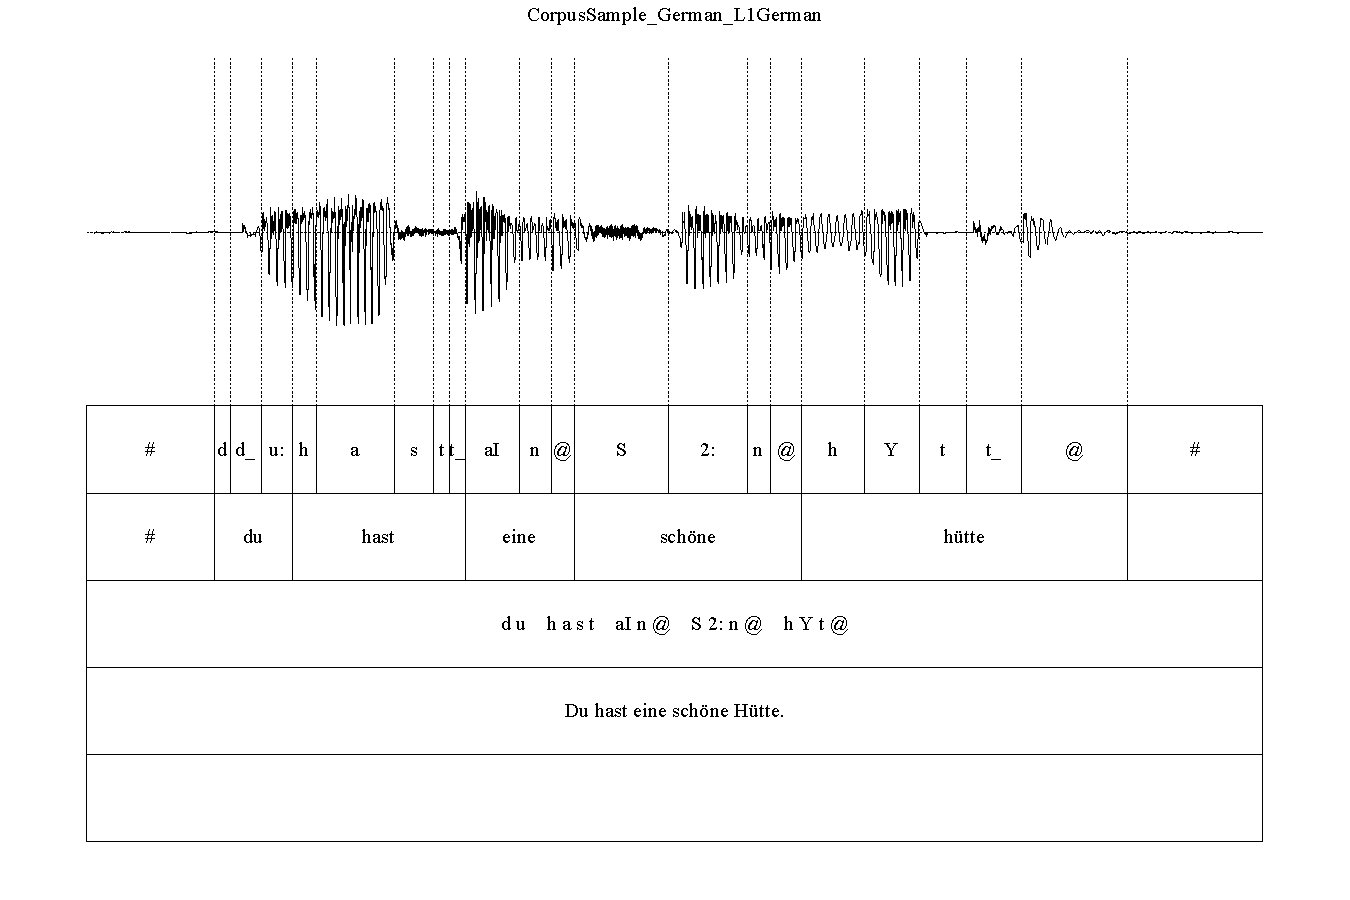
\includegraphics[width=\textwidth]{img/screenshots/SampleGG-basic}
		\caption[An example German utterance and its segmentation]{\TODO{update with new example w/ SyllableTier} An example of a German utterance that has been segmented at the phone level (first row) and word level (second row). The third row contains the canonical (expected) native pronunciation of each word in the sentence, while the fourth row contains the written sentence of which the utterance is a reading.}
		\label{fig:GGsegmentation}
	\end{figure}


A reasonably accurate segmentation of an L2 learner's utterance is indispensable for an analysis of the accuracy of their pronunciation; 
\TODO{mention that there are methods which don't need segmentation, but they're more limited?}
as it allows comparison between relevant units of the learner's utterance -- e.g. words, syllables, and phones -- and corresponding units in native speech. 
The most accurate segmentation would of course be one produced by hand by a trained phonetician. However, hand-labeling is not feasible in most scenarios because of its high cost in terms of time and wages; moreover, because the ultimate goal of this work is the development of a CAPT tool which can give L2 learners helpful automatic feedback on their pronunciation, 
%even when they do not have access to a language teacher, 
any analysis of the learner's speech signal, including the preliminary step of segmentation, must proceed fully automatically. Therefore, a means of automatically segmenting a given utterance is required.



	%\subsection{Segmentation via forced alignment}
	%\label{sec:segmentation:alignment}
	
	When the content (text) of a given utterance is already known, the goal of automatic segmentation becomes aligning the  boundaries of each phone in the expected sentence with the appropriate points in the recorded signal. Boundaries for larger units such as syllables and words can be inferred from the phone boundaries. 
	An effective and widely-used technique for this is forced
	% (Viterbi) 
	alignment \citep{Fohr1996,Mesbahi2011,Fohr2012,Fauth2014}.
	%which uses the Viterbi algorithm to 
	%
	This technique 
	requires:
	\begin{itemize}
%knowledge of the text of the given utterance (known beforehand in the IFCASL case), 
	\item the expected text (word sequence) of the given utterance, 
	\item a pronunciation lexicon containing the sequence of phones expected for each word, and
	\item an acoustic model for the target language.
	%which captures how phones in the target language (and potentially other phenomena, e.g. breathing or silence) are realized acoustically.
	\end{itemize}
	
	The first of these requirements, the text of the utterance, is trivial when the speaker has been asked to read a given sentence aloud, which is the case in \TODO{this context \textit{is that unclear?}}.
	%
	A lexicon of canonical word pronunciations, i.e. the pronunciations that might be given in a standard dictionary, is also relatively easy to obtain for a well-researched language such as German, for which many digital linguistic resources exist.
	 To account for differences in how different speakers (especially non-native speakers) may pronounce the given sentence, 
	%the lexicon is supplemented with a lexicon of non-native pronunciation variants 
	the lexicon should contain not only the canonical pronunciation for each word, but also any alternate or non-standard pronunciation variants (native or non-native) that might be encountered. Research \TODO{at LORIA} has found the inclusion of non-native pronunciation variants to lead to improvements in the accuracy of automatic segmentation of non-native speech \citep{Jouvet2011,Mesbahi2011,Bonneau2012,Orosanu2012}, and one of the intended outcomes of the IFCASL project is the extraction of a non-native variant lexicon from the L2 speech in the corpus \TODO{ref?}.
	
	The final requirement for segmentation via forced alignment is an acoustic model, i.e. a statistical model 
	%(typically a Hidden Markov Model) 
	%trained on speech in the target language 
	which captures the correspondence between acoustic features extracted from the speech signal and phones in the target language. 
	To accurately capture this correspondence, the model must be trained on a large amount of speech data in the target language; 
	the acoustic model used to align the German IFCASL data was trained on native German speech from the Kiel corpus \TODO{ref, verify}.
	However, research by \citeauthor{Bouselmi2005} (\citeyear{Bouselmi2005,Bouselmi2012}) has shown that even more accurate segmentation of learners' utterances an be obtained by using acoustic models adapted to non-native speech in the target language and/or speech in the learner's L1; refining the automatic segmentation functionality using such adapted models would therefore be a logical extension of this work (see \cref{sec:conclusion:future}) \TODO{does that clause work?}.
	
	\TODO{Details about how forced Viterbi alignment works?}
	%Given the expected text and the corresponding phone sequence, forced alignment consists of using the Viterbi algorithm and an acoustic Hidden Markov Model trained on the target language to determine the temporal locations of boundaries between each of the expected phones. The Viterbi algorithm is commonly used in automatic speech recognition to determine... 

	
	Given these resources, the Jsnoori software,
	\TODO{\textit{awkward:}} which the lexical stress CAPT tool developed in this work uses for speech processing,
	%used to process speech in the lexical stress CAPT tool
	is capable of automatically segmenting a learner's utterance almost instantly. Unfortunately, a disadvantage of forced alignment is that it requires the entire utterance (e.g. sentence), so real-time segmentation is not possible \TODO{true? should this go in a footnote?}. However, acoustic models and pronunciation lexicons for German have yet to be integrated into Jsnoori, which 
	%is currently only capable of segmenting 
	currently only has the resources to segment 
	speech in English and French.
	 %In the absence of automatic segmentation capabilities for German,
	 Therefore,
	 the prototype CAPT tool developed in this thesis project presupposes the existence of a segmentation for a given utterance,
	%the tool %thus takes 
	taking a ``Wizard-of-Oz'' approach to the automatic segmentation step by demonstrating its error diagnosis and feedback capabilities using learner (L2) and reference (L1) read-speech utterances from the German-language subset of the IFCASL corpus \citep{Fauth2014,Trouvain2013}, all of which have been segmented at the phone and word levels using the forced alignment technique described above.
	Once the requisite German-language resources are available in Jsnoori, the tool can easily be extended to perform on-the-fly segmentation of learner utterances (see \cref{sec:conclusion:future}).
	
	%\TODO{a real CAPT system would have to do this on the fly, and that can be done in Jsnoori, but the prototype assumes segmentation has been done and mocks that up by only using auto segmentations of IFCASL data}
	%
	
	
	\TODO{\textit{awkward clause:}} Although the IFCASL corpus also contains manually-corrected versions of the majority of the forced-alignment segmentations,
	the CAPT tool only makes use of the automatically-determined determined boundaries, even though these are potentially less accurate; 
	this is to more accurately 
	%reflect the fact that any 
	simulate the conditions of a 
	fully-automatic CAPT system,
	which 
	would need to perform segmentation on the fly without recourse to manual verification.
	%The native and non-native read speech recordings comprising the German-language subset of the IFCASL corpus \citep{Fauth2014,Trouvain2013} have already been automatically segmented via forced alignment, as described above.
	%\TODO{paragraph break?}
	Indeed, 
	%segmentations obtained by forced alignment 
	forced alignment is not a perfect method; \TODO{\textit{unclear?:} because of the constraints put on the recognition system,} the aligner will always find a match between the given text and audio, even if they do not correspond.  
	Therefore, inaccuracies in the phone boundaries determined using this technique should be expected, especially when the alignment is performed on non-native utterances using an acoustic model trained on native speech.
		\TODO{Reliability of non-native speech automatic segmentation for prosodic feedback. \citep{Mesbahi2011}}
		\TODO{\textit{work this sentence in somewhere:}} A fully-fledged CAPT system extending this thesis project would have to cope with any problems that may result from using imperfect automatic segmentations as a starting point for analysis.
	
	
	As mentioned above, the utterances in the IFCASL corpus have %pre-existing 
	segmentations at the phone and word levels; however, the corpus does not contain syllable-level segmentations.
	%but not at the syllable level.
	%and a subset of these automatic segmentations has been manually verified.
	As the syllable is arguably the most important unit for analysis of lexical stress realization \TODO{reference/justification}, syllable-level segmentations had to be created for each utterance. This was accomplished by 
	 %However, segmentation at the syllable level still needs to be performed. This may be accomplished based on the word- and phone-level annotations by automatically or 
	 manually determining the locations of syllable boundaries in the phone sequence for each word, 		%(i.e. the locations in the phone sequence where syllable boundaries are expected) 
	 %using the text of each sentence and a syllabified phonetic lexicon from the speech synthesis system MaryTTS \citep{Schroeder2003}, 
	%\TODO{using the syllabification program [...] and a pronunciation dictionary?  },
	 %Given the sequence of phones expected for each syllable, the locations of syllable boundaries were automatically extracted 
	 %using  to 
	 automatically extracting the temporal locations of these %syllable 
	 boundaries
	 from the phone-level segmentation, 
	 and automatically combining the word-internal syllable boundaries with the boundaries in the word-level segmentation to create the syllable-level segmentation. 


	

	
%%%%%%%%%%%%%%%%%%%%%%%
%%% Moved to Future Work
%%%%%%%%%%%%%%%%%%%%%%%
	%\subsection{Evaluation of segmentation accuracy}
	%\label{sec:segmentation:eval}
%	
%	The accuracy of the forced-alignment segmentation can be assessed by computing inter-annotator agreement between the automatically produced segmentation and one or more manually-verified segmentations. The team at LORIA in Nancy has already completed this evaluation for the French IFCASL sub-corpus using the CoALT tool \citep{Fohr2012}. In cooperation with that team, the German sub-corpus (or a subset thereof) will be evaluated in the same way.
%	A similar evaluation will be carried out for the syllable-level segmentations, a subset of which will be manually verified.
%
%%	Error analysis will be performed for each boundary type, to enable identification of the types of boundaries at which the system tends (not) to make many errors. This detailed analysis will contribute to error management in the system, as described 
%%in \cref{sec:segmentation:errors}.
%%below.

%	\subsection{Coping with segmentation errors}
%	\label{sec:segmentation:errors}
%	
%	Forced alignment is not a perfect method; because of the constraints put on the recognition system, the aligner will always find a match between the given text and audio, even if they do not correspond. Incorrect segmentation can lead to mistakes in diagnosis, so CAPT systems must have a means of reducing, or at least monitoring, the amount of error introduced by inaccurate segmentation \citep{Eskenazi2009}. 	
%	In the proposed CAPT tool, this function may be served by the development of a simple sentence- and/or word-level confidence measure. 
%	While it is very difficult to compute such a measure directly from the decoding scores of the forced aligner, it may be possible to determine from the aforementioned accuracy evaluation which types of boundaries (e.g. between a sonorant and a vowel) the aligner typically has trouble detecting accurately, and then to calculate, for a given utterance, the proportion of error-prone boundaries. While a very simplistic measure, this could nevertheless provide some indication of when (not) to trust the automatic alignment, thus impacting decisions on how and whether to attempt error diagnosis (or feedback).
%	% based on the boundary error rates found in \cref{sec:segmentation:eval}. 
%	Other error-management strategies may also be explored, such as the type of error-filtering methods described by \textcite{Mesbahi2011,Bonneau2012,Orosanu2012}, in which utterances which do not correspond to the expected text are detected and rejected before alignment is attempted.
%%%%%%%%%%%%%%%%%%%%%%%
	
\section{Analysis of word prosody}
\label{sec:diag:prosody}

	\TODO{Technically these features aren't all relevant to comparison-based diagnosis, only classification - so I guess this whole section needs to be rewritten :/}
	
	The automatically-determined word, syllable, and phone boundaries obtained as described in the previous section 
	%were used to 
	enable the CAPT tool to locate and analyze segments of the speech signal relevant to the realization of lexical stress.
	%, enabling analysis of these  
	%in terms of the acoustic correlates of word prosody described in \cref{sec:background:stress}.  
	This section describes the features by which the system analyzes the lexical stress prosody of an utterance, be it the utterance of a learner or of a native speaker. These features relate to the three \TODO{acoustic properties (and by extension their perceptual correlates)} described in \cref{sec:bkgd:stress}, namely duration (timing), fundamental frequency (pitch), and intensity (loudness). 
		%The features computed for each property are described in the corresponding sections below.
%
	%\TODO{Where possible, the diagnosis module of the CAPT tool will provide researchers control over the features used; for example, there may be an option to include all F0 and duration features but ignore intensity features.}
%	

%TODO {\textit{To go somewhere in this section:} Added German phonetic inventories to Jsnoori so that it could know e.g. which segments are vowels}


	Throughout this section, the features discussed are illustrated with their values for a word from \TODO{\textit{three?} two sample utterances} of a German word selected from the IFCASL corpus; one by a L1 French speaker and the other by a L1 German speaker. The oscillogram, waveform, and annotation for these samples are shown in \cref{fig:featuresexample}.
	
	\begin{figure}
		\centering
		\begin{subfigure}[t]{\textwidth}
                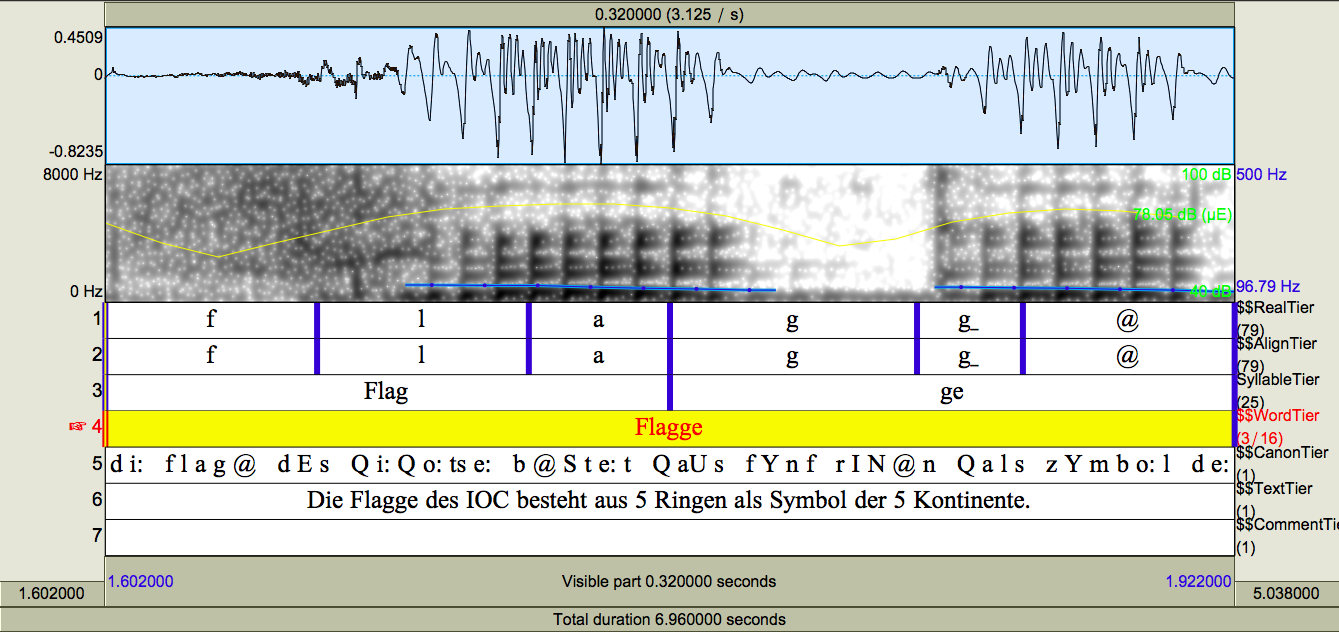
\includegraphics[width=\textwidth]{img/screenshots/2SH05_FGMB1_527-flagge}
                \caption{L1 French speaker (F)}
                \label{fig:featuresexample:fg}
        \end{subfigure}%
        \vspace{1.5em}
        \TODO{Add incorrect FG example?}        \vspace{1.5em}

        \begin{subfigure}[b]{\textwidth}
                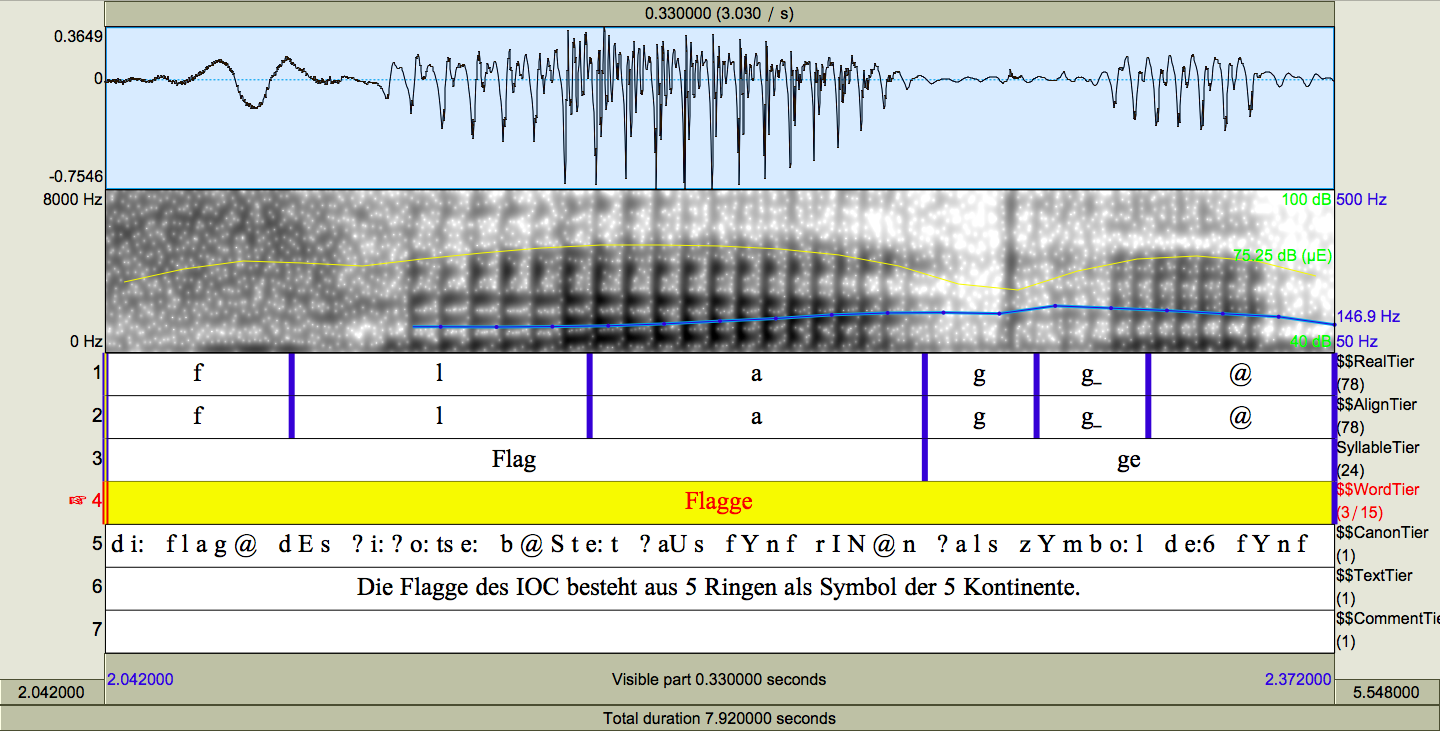
\includegraphics[width=\textwidth]{img/screenshots/2SH05_GGMB2_035-flagge}
                \caption{L1 German speaker (G)}
                \label{fig:featuresexample:gg}
        \end{subfigure}%
		\caption{Two sample utterances of the word "Flagge" from the IFCASL corpus, used to illustrate the features discussed in this section. \TODO{description}}
		\label{fig:featuresexample}
	\end{figure}
	
Once again it should be stressed that the features described below are computed from the automatically generated segmentation of a given utterance, and not from a hand-corrected segmentation; as a result, the computed values may be slightly (or in some cases, significantly) inaccurate due to errors in the forced-alignment segmentation process, as just discussed in \cref{sec:diag:segmentation}. %MOVED ABOVE This reliance only on automatically-detected segment boundaries is intentional, as it simulates the conditions of an automatic, real-time tutoring system, which would need to perform segmentation on the fly and would not have recourse to human verification of segment boundary locations.
	%
	\TODO{\textit{Worth mentioning? Seems a bit out of place}} 
	%A potential complication of this analysis that should be pointed out relates to 
	Also worth noting is the fact that we are here dealing exclusively with read, and not sponaneous, speech. As \textcite[p.~275]{Cutler2005} remarks, ``acoustic differences between stressed and unstressed syllables are relatively large in spontaneous speech. With laboratory-read materials, however, such differences do not always arise''. Therefore, the task of recognizing prosodic deviations in learners' read speech may be somewhat different than the corresponding task for spontaneous speech, and this difference should be kept in mind in the discussion that follows.

	\subsection{Duration}
	\label{sec:prosody:duration}
	%TODO more text
	Analysis of duration (timing) is extremely important for detecting stress patterns;
indeed, syllable duration may be the most important acoustic correlate of lexical stress in German \citep{Dogil1999}.
%as discussed in section %TODO above.
%In this work, duration analysis will figure prominently, and following \textcite{Bonneau2011} will most likely take into account the relative duration of each syllable of the word in question, and/or of the vowel at the nucleus of each syllable. %Other features may also be explored.
Duration analysis therefore figures prominently in the analysis and assessment of learners' lexical stress in this work. 


Given the word-, syllable- and phone-level segmentations of an utterance (see \cref{sec:diag:segmentation}), the extraction of duration features for that utterance is trivial, as it consists simply of noting the duration of each relevant segment. % in the appropriate segmentation. 
Following \textcite{Bonneau2011}, \TODO{we} take into account the %relative
 duration of each syllable in the word to be analyzed, and
 %as well as the %relative duration 
 of the vowels at the nucleus of each syllable. 
 	\TODO{Mention that to find vowels I had to add German phonetic inventory to Jsnoori?}
	To account for inter-speaker variability, e.g. the fact that some speakers may have an overall slower or faster speech rate than others, relative rather than absolute durations are used.
	The list of duration features computed for each word utterance is given in \cref{tab:durationfeatures}, 
along with the values computed for each feature from the sample utterances shown in \cref{fig:featuresexample}. % from the IFCASL corpus \TODO{reference?}. 


\begin{table}[htb]
		\centering
		\caption[Features computed for duration analysis]{Features computed for duration analysis, and their values for the sample utterances of ``Flagge'' in \cref{fig:featuresexample}. Values are given in seconds. \TODO{remove absolutes}}
		
		\begin{subtable}[h]{\textwidth}
		\caption{Absolute features}
		\begin{tabularx}{\textwidth}{lXcc}
		\toprule
		\multirow{2}{*}{Feature name} 
									& \multirow{2}{*}{Description}
																	& \multicolumn{2}{c}{Value (seconds)} \\
					  				&												&  (a) F		& (b) G \\
		\midrule
		WORD-DUR 		&	Duration of entire word \TODO{remove?}				& 0.32			& 0.33			\\
		SYLL0-DUR 		&	Dur. of 1st syllable						& 0.16			& 0.22			\\
		SYLL1-DUR 		&	Dur. of 2nd syllable				& 0.16			& 0.11			\\
		V0-DUR 				&	Dur. of vowel in 1st syllable		& 0.04			& 0.09			\\
		V1-DUR 				&	Dur. of vowel in 2nd syllable	& 0.06			& 0.05			\\
		\bottomrule
		\end{tabularx}
		\end{subtable}

		\vspace{1em}		
		
		\begin{subtable}[h]{\textwidth}
		\caption{Relative features}
		\begin{tabularx}{\textwidth}{lXcc}
		\toprule
		\multirow{2}{*}{Feature name} 
									& \multirow{2}{*}{Description}
														& \multicolumn{2}{c}{Value} \\
	&												&  (a) F		& (b) G \\
		\midrule
		REL-SYLL-DUR 	&	SYLL1-DUR$/$SYLL0-DUR 		& 1.00			& 2.00			\\
		REL-V-DUR 		&	V1-DUR$/$V0-DUR					& 0.67			& 1.80 			\\
		\bottomrule	
		\end{tabularx}
		\end{subtable}
		\label{tab:durationfeatures}
\end{table}

The relative utility of these features in automatically diagnosing lexical stress errors is discussed further in \cref{sec:diag:eval}.


	\subsection{Fundamental frequency}
	\label{sec:prosody:f0}
	
	As described in \cref{sec:bkgd:stress}, the fundamental frequency (F0) of an utterance, which corresponds at the perceptual level to its pitch, also provides a strong indication of how lexical stress is realized in that utterance, and F0 features 
	%should therefore also contribute to 
	are another crucial component of
	the system's prosodic analysis. 
	%
	
		\TODO{Pitch in Jsnoori:
	\begin{itemize}
		\item Martin's basic spectral comb algo
		\item with Yves' improvement using parabolic interpolation
		\item with Secrest \& Doddington's improvement for voicing decision 
		\item With dynamic programming (Ney?) to select which F0 values to accept
		\item Soon to implement Yin's temporal method, and then combine results with those of Martin's or another spectral method such as SWIPE (SWYPE?) (combining with NNs or something else)
		\item semitones
		\item 0 values are excluded from mean calculations
	\end{itemize}	
	}	
	
	The F0 contour of a given utterance is determined using the pitch detection algorithm(s) implemented in Jsnoori \TODO{ref}. At the heart of Jsnoori's approach to pitch detection lies the algorithm developed by \textcite{Martin1982}, which \TODO{...}
	
	\TODO{de-proposal-ize this paragraph}
	Much of the work on assessing non-native lexical stress has been conducted with English as the L2, and thus often makes the assumption that a stressed syllable should have a higher F0 than unstressed syllables \citep{Bonneau2011}. In German, the F0 of a stressed syllable also tends to differ from the surrounding contour, but the difference may be positive (the stressed syllable has a higher pitch than surrounding syllables) or negative (lower pitch) \citep[p.~267]{Cutler2005}. 		%``...in German utterances, stressed syllables could be signaled by any F0 obtrusion from the overall contour, so that a stressed syllable could be either higher or lower in pitch than its neighbors'' \citep[p.~267]{Cutler2005}
	Therefore, the computed features
	%include not only the difference in F0 maxima between syllables in the word and the location (syllable index) of the word's F0 maximum, but also the analogous features for F0 minima and ranges.
	capture not only the F0 maximum of each syllable, but also the minimum and range (difference between maximum and minimum) \TODO{more/separate discussion of why range might be important?}.
	 
	%To guard against unvoiced segments interfering with the F0 analysis, syllables may be represented by the vowels that form their nuclei. Relative differences between syllables may be more helpful than absolute differences. The F0 variation (range) over the entire word might also be informative of whether or not the speaker failed to stress any syllable.%, although it would not tell us which syllable were stressed. 
	%Other features may be drawn from related work on lexical stress in learner speech, such as \textcite{Bonneau2011}.
	


		%\setlength\extrarowheight{5pt}
\begin{table}[htb]
		\centering
		\caption[Features computed for fundamental frequency (F0) analysis]{Features computed for fundamental frequency (F0) analysis, and their values for the sample utterances of ``Flagge'' in \cref{fig:featuresexample}.% Values are given in semitones.
		}
		{\renewcommand{\arraystretch}{1.4}%
		
		\begin{subtable}[h]{\textwidth}
		\caption{Absolute features}
		\begin{tabularx}{\textwidth}{p{.225\textwidth}Xrr}
		\toprule
		\multirow{3}{*}{Feature name} 
									& \multirow{3}{*}{Description}
																	& \multicolumn{2}{c}{Value} \\
									&								& \multicolumn{2}{c}{(semitones)} \\							
					  				&																	&  (a) F		
					  																											& (b) G
					  																																\\
		\midrule
		%%%% WORD FEATURES 
		WORD-F0-MEAN	& Average (Avg.) F0, entire word	 				& 8.78		& 16.36\\
		WORD-F0-MAX	& Maximum (Max.) F0, entire word				& 10.73	& 20.08\\
		WORD-F0-MIN		& Minimum (Min.) F0, entire word				& 6.27		& 13.65\\
		WORD-F0-RANGE & WORD-F0-MAX$-$WORD-F0-MIN			& 4.46		& 6.43\\
%		WORD-F0-RANGE & {\renewcommand{\arraystretch}{.9}%
%										$\displaystyle\begin{array}{l}%
%										\phantom{-}\mbox{WORD-F0-MAX}\\%
%										-\mbox{WORD-F0-MIN}\\\end{array}$}	& 4.46	& 6.43\\
%		\multirow{2}{*}{WORD-F0-RANGE}	
%									& $\phantom{- }\text{WORD-F0-MAX}$
%																			& \multirow{2}{*}{4.459217}		
%																									& \multirow{2}{*}{6.425775}\\
%									& $- \text{WORD-F0-MIN}$						& 						& 					\\		

		%\addlinespace
		%%%% SYLL* FEATURES 
		SYLL0-F0-MEAN	& Avg. F0, 1st syllable					& 9.29		& 15.81\\	
		V0-F0-MEAN		& Avg. F0, 1st syllable	nucleus				& \color{red}{TD}		& \color{red}{TD}\\
		SYLL0-F0-MAX		& Max. F0, 1st syllable					& 10.73		& 18.25\\
		V0-F0-MAX		& Max. F0, 1st syllable	nucleus				& \color{red}{TD}		& \color{red}{TD}\\
		SYLL0-F0-MIN		& Min. F0, 1st syllable					& \color{red}{TD}		& \color{red}{TD}\\
		V0-F0-MIN		& Min. F0, 1st syllable	nucleus				& \color{red}{TD}		& \color{red}{TD}\\
		SYLL0-F0-RANGE & SYLL0-F0-MAX$-$SYLL0-F0-MIN	& 1.45		& 4.60\\
		V0-F0-RANGE		& V0-F0-MAX$-$V0-F0-MIN				& \color{red}{TD}		& \color{red}{TD}\\
%		SYLL0-F0-RANGE	& {\renewcommand{\arraystretch}{.9}%
%										$\displaystyle\begin{array}{l}%
%										\phantom{-}\mbox{SYLL0-F0-MAX}\\%
%										-\mbox{SYLL0-F0-MIN}\\\end{array}$} 		& 1.45		& 4.60\\
%		\multirow{2}{*}{SYLL0-F0-RANGE}	
%									& $\phantom{- }\text{SYLL0-F0-MAX}$%-$SYLL0-F0-MIN	
%																			& \multirow{2}{*}{1.44952}		
%																										& \multirow{2}{*}{4.600318}\\
%									& $- \text{SYLL0-F0-MIN}$					& 						& 					\\		

		SYLL1-F0-MEAN	& Avg. F0, 2nd syllable						& 8.24		& 17.51\\
		V1-F0-MEAN		& Avg. F0, 2nd syllable	nucleus				& \color{red}{TD}		& \color{red}{TD}\\
		SYLL1-F0-MAX		& Max. F0, 2nd syllable						& 9.93		& 20.08\\
		V1-F0-MAX		& Max. F0, 2nd syllable	nucleus				& \color{red}{TD}		& \color{red}{TD}\\
		SYLL1-F0-MIN		& Min. F0, 2nd syllable			& \color{red}{TD}	& \color{red}{TD}\\
		V1-F0-MIN		& Min. F0, 2nd syllable 	nucleus				& \color{red}{TD}		& \color{red}{TD}\\
		SYLL1-F0-RANGE	& SYLL1-F0-MAX$-$SYLL1-F0-MIN 	& 3.66		& 5.86 \\
		V1-F0-RANGE		& V1-F0-MAX$-$V1-F0-MIN				& \color{red}{TD}		& \color{red}{TD}\\
%		SYLL1-F0-RANGE	& {\renewcommand{\arraystretch}{.9}%
%										$\displaystyle\begin{array}{l}%
%										\phantom{-}\mbox{SYLL1-F0-MAX}\\%
%										-\mbox{SYLL1-F0-MIN}\\\end{array}$} 		& 3.66	& 5.86 \\
%		\multirow{2}{*}{SYLL1-F0-RANGE}	
%									& $\phantom{- }\text{SYLL1-F0-MAX}$%-$SYLL1-F0-MIN	
%																			& \multirow{2}{*}{3.65978}		
%																										& \multirow{2}{*}{5.862722}\\
%									& $- \text{SYLL1-F0-MIN}$					& 						& 					\\		
		
		%\addlinespace
		\bottomrule
		\end{tabularx}
		\end{subtable}
		}
		\end{table}
		%\vspace{1em}
		
		\begin{table}[ht]
		\ContinuedFloat
		\caption[Features computed for fundamental frequency (F0) analysis (cont.)]{(continued) Features computed for fundamental frequency (F0) analysis, and their values for the sample utterances of ``Flagge'' in \cref{fig:featuresexample}.% Values are given in semitones.
		}
		\begin{subtable}[h]{\textwidth}
		\caption{Relative features}
		\begin{tabularx}{\textwidth}{p{.225\textwidth}Xrr}
		\toprule
		\multirow{2}{*}{Feature name} 
									& \multirow{2}{*}{Description}
													& \multicolumn{2}{c}{Value} \\						
					  				&							&  (a) F		& (b) G
					  																																\\
		\midrule
		%%%% RELATIVE FEATURES 
%		SYLL-REL-MEAN & {\renewcommand{\arraystretch}{.9}%
%									 $\displaystyle\begin{array}{l}
%									 \mbox{SYLL0-F0-MEAN}\\
%									 \hline
%									 \mbox{SYLL1-F0-MEAN}\\
%									 \end{array}$}			
%																				& 1.12688     & 0.903218 \\		
		REL-SYLL-F0-MEAN & SYLL0-F0-MEAN$/$SYLL1-F0-MEAN 	& 1.13    & 0.90 \\
		REL-V-F0-MEAN & V1-F0-MEAN$/$V0-F0-MEAN &  \color{red}{TD}	& \color{red}{TD}\\
%		SYLL-REL-MEAN
%							& $\displaystyle\frac{\mbox{SYLL0-F0-MEAN}}{\mbox{SYLL1-F0-MEAN}}$			
%																									& 1.13    & 0.90 \\
		%\addlinespace
		REL-SYLL-F0-MAX & SYLL1-F0-MAX$/$SYLL0-F0-MAX 			& 1.08		& 0.91 \\
		REL-V-F0-MAX & V1-F0-MAX$/$V0-F0-MAX &  \color{red}{TD}	& \color{red}{TD}\\
%		SYLL-REL-MAX
%							& $\displaystyle\frac{\mbox{SYLL0-F0-MAX}}{\mbox{SYLL1-F0-MAX}}$
%																									& 1.08		& 0.91 \\
		REL-SYLL-F0-MIN & SYLL1-F0-MIN$/$SYLL0-F0-MIN &\color{red}{TD}&\color{red}{TD}\\
		REL-V-F0-MIN & V1-F0-MIN$/$V0-F0-MIN &  \color{red}{TD}	& \color{red}{TD}\\
		
		%\addlinespace
%		SYLL-REL-MIN		
%							& $\displaystyle\frac{\mbox{SYLL0-F0-MIN}}{\mbox{SYLL1-F0-MIN}}$	
%																		& \color{red}{TD}		& \color{red}{TD}\\
		%\addlinespace
		REL-SYLL-F0-RANGE & SYLL1-F0-RANGE$/$SYLL0-F0-RANGE & 0.40%0.396068		
																															& 0.78\\
																															REL-V-F0-RANGE & V1-F0-RANGE$/$V0-F0-RANGE &  \color{red}{TD}	& \color{red}{TD}\\
%		SYLL-REL-RANGE	
%							& $\displaystyle\frac{\mbox{SYLL0-F0-RANGE}}{\mbox{SYLL1-F0-RANGE}}$
%																									& 0.40%0.396068		
%																															& 0.78\\
		%\addlinespace
		F0-MAX-INDEX	
							& 	$\begin{cases} 
								0, & \text{if SYLL0-F0-MAX}>\text{SYLL1-F0-MAX}\\
								1, & \text{if SYLL0-F0-MAX}<\text{SYLL1-F0-MAX}\\
								\end{cases}$
%							& 0 if  SYLL0-F0-MAX$>$SYLL1-F0-MAX,
%								1 if  SYLL0-F0-MAX$<$SYLL1-F0-MAX		
																									& 0					& 1				\\
		F0-MIN-INDEX	
							& 	$\begin{cases} 
								0, & \text{if SYLL0-F0-MIN}<\text{SYLL1-F0-MIN}\\
								1, & \text{if SYLL0-F0-MIN}>\text{SYLL1-F0-MIN}\\
								\end{cases}$
%							& 0 if  SYLL0-F0-MIN$<$SYLL1-F0-MIN,
%								1 if  SYLL0-F0-MIN$>$SYLL1-F0-MIN		
																									& 1					& 0				\\
																									
		F0-MAXRANGE-INDEX	
					& $\begin{cases} 
								0, & \text{if SYLL0-F0-RANGE}>\text{SYLL1-F0-RANGE}\\
								1, & \text{if SYLL0-F0-RANGE}<\text{SYLL1-F0-RANGE}\\
							\end{cases}$
%					& 0 if  SYLL0-F0-RANGE$>$SYLL1-F0-RANGE,
%						1 if  SYLL0-F0-RANGE$<$SYLL1-F0-RANGE		
																									& 1					& 1				\\
		\bottomrule
		\end{tabularx}
		\end{subtable}
		
%		} % end arraystretch
		\label{tab:durationfeatures}
\end{table}


	\subsection{Intensity}
	\label{sec:prosody:intensity}
	
	\TODO{Energy in Jsnoori:
	\begin{itemize}
		\item Determined by FFT
		\item Which window size/spacing used?
		\item Energy calculated in which frequency band (range)?
		\item Other parameters for energy calc?
	\end{itemize}
	}	
	
		Research on lexical stress prosody has generally indicated that intensity is the least important of the three features, i.e. corresponds least closely to lexical stress patterns \citep{Cutler2005}. 
Indeed, existing lexical stress assessment tools may not take intensity into account, as is the case in the system described by \textcite{Bonneau2011}.  However, intensity can nonetheless have an impact on the perception of lexical stress, especially in combination with pitch or duration, or both \citep{Cutler2005}; %TODO check this reference
Therefore, the diagnosis system should ideally take intensity into account when performing its prosodic analysis. This could be as simple as computing the total energy of the part of the signal corresponding to each syllable of the word in question, although more complex measures may be explored if time allows.
	
	
\begin{table}[htb]
		\centering
		\caption[Features computed for intensity  analysis]{Features computed for intensity analysis, and their values for the sample utterances of ``Flagge'' in \cref{fig:featuresexample}.}	
		
		
		\begin{subtable}[h]{\textwidth}
		\caption{Absolute features}
		\begin{tabularx}{\textwidth}{p{.3\textwidth}Xrr}
		\toprule
		\multirow{3}{*}{Feature name} 
							& \multirow{3}{*}{Description}
									& \multicolumn{2}{c}{Value} \\
							&		& \multicolumn{2}{c}{(\TODO{units})} \\							
					  		&		&  (a) F		& (b) G\\
		\midrule
		
	
WORD-ENERGY-MEAN & \color{red}{TD} &  \color{red}{TD}	& \color{red}{TD}\\
WORD-ENERGY-MAX & \color{red}{TD} &  \color{red}{TD}	& \color{red}{TD}\\
SYLL0-ENERGY-MEAN & \color{red}{TD} &  \color{red}{TD}	& \color{red}{TD}\\
SYLL0-ENERGY-MAX & \color{red}{TD} &  \color{red}{TD}	& \color{red}{TD}\\
SYLL1-ENERGY-MEAN & \color{red}{TD} &  \color{red}{TD}	& \color{red}{TD}\\
SYLL1-ENERGY-MAX & \color{red}{TD} &  \color{red}{TD}	& \color{red}{TD}\\
V0-ENERGY-MEAN & \color{red}{TD} &  \color{red}{TD}	& \color{red}{TD}\\
V0-ENERGY-MAX & \color{red}{TD} &  \color{red}{TD}	& \color{red}{TD}\\
V1-ENERGY-MEAN & \color{red}{TD} &  \color{red}{TD}	& \color{red}{TD}\\
V1-ENERGY-MAX & \color{red}{TD} &  \color{red}{TD}	& \color{red}{TD}\\
	
	\bottomrule
	\end{tabularx}
	\end{subtable}
	
\end{table}

\begin{table}[ht]
	\ContinuedFloat
	\caption[Features computed for intensity analysis (cont.)]{(continued) Features computed for intensity analysis, and their values for the sample utterances of ``Flagge'' in \cref{fig:featuresexample}.}	
		
	\begin{subtable}[h]{\textwidth}
	\caption{Relative features}
	\begin{tabularx}{\textwidth}{p{.35\textwidth}Xrr}
	\toprule
	\multirow{2}{*}{Feature name} 
					& \multirow{2}{*}{Description}
										& \multicolumn{2}{c}{Value} \\	
				  	&							&  (a) F		& (b) G			\\
	\midrule
	
REL-SYLL-ENERGY-MEAN & \color{red}{TD} &  \color{red}{TD}	& \color{red}{TD}\\
REL-SYLL-ENERGY-MAX & \color{red}{TD} &  \color{red}{TD}	& \color{red}{TD}\\
REL-VOWEL-ENERGY-MEAN & \color{red}{TD} &  \color{red}{TD}	& \color{red}{TD}\\
REL-VOWEL-ENERGY-MAX & \color{red}{TD} &  \color{red}{TD}	& \color{red}{TD}\\
ENERGY-MAX-INDEX & \color{red}{TD} &  \color{red}{TD}	& \color{red}{TD}\\
	
	\bottomrule
	\end{tabularx}
	\end{subtable}
	
\end{table}
	
	
\section{Diagnosis by direct comparison}
%\section{Comparison of native and nonnative speech}
\label{sec:diag:compare}

	This thesis will explore a variety of approaches to modeling the lexical stress prosody of native speech in such a way that the learner's utterance can be automatically compared to that native model. This investigation, and the creation of a CAPT tool that allows researchers to easily switch between approaches to study their effects, will be one of the primary contributions of the thesis.
	
	\subsection{Using a single reference speaker}
	\label{sec:compare:single}
	
	The most common approach to assessing L2 prosody involves comparing a learner's utterance to the same utterance produced by a native speaker of the target language; this approach is taken by \textcite{Bonneau2011} and others.% \citep{Eskenazi2009, Delmonte2011}. %TODO take that citation out?
%	 Inspired and informed by the investigations of \textcite{Probst2002}, this work will examine different ways of selecting the reference speaker against which a learner's utterance will be judged, given a pool of potential references. 


	\subsection{Using multiple reference speakers}
	\label{sec:compare:multi}
	
	However, when using a single native-speaker utterance for reference, even if the chosen speaker has been chosen carefully, we may be ``over-fitting'' to speaker- or utterance-dependent characteristics of the reference utterance that do not accurately represent the ``nativeness'' of the reference speech. It would therefore be advantageous not to limit the diagnosis to comparison with a single reference speaker, but to instead compare the learner's speech with a variety of native utterances. This could be accomplished by conducting a series of one-on-one comparisons, pairing the learner utterance with a different reference utterance for each comparison, and then combining the results from all the comparisons.  Factors to explore in this approach might include whether the set of reference speakers should be more or less constrained (e.g. by gender), and which metrics can be used to synthesize the one-on-one comparisons into a single diagnosis.
	
%TODO replace?
%	Alternatively, the learner's utterance could perhaps be compared directly with some unified representation of all the reference utterances; for example, if we represent each reference utterance as a point in n-dimensional space, with each dimension representing a relevant feature, the references will form a cluster which can serve as a representation of the variation permissible in native speech. By plotting the learner's utterance in the same space, it could be possible to distinguish how well (or poorly) this utterance fits into that cluster, and thereby produce a diagnosis.

	\subsection{Reference speaker selection}
	\label{sec:compare:selection}	
	
		\subsubsection{Manually selecting a reference}
		\label{sec:selection:manual}
		%\label{sec:compare:single:manual}
		
		The most basic way of selecting a reference speaker is to choose one manually.
%manually specify which speaker should be used for comparison. 
As a type of baseline, the CAPT tool will therefore enable the learner and/or the instructor/experimenter to choose a reference from a set of available speakers, with that set potentially being constrained by one or more properties of the speaker (e.g. gender). 
	
		\subsubsection{Automatically selecting a reference}
		\label{sec:selection:auto}
		%\label{sec:compare:single:auto}
		
		Another means of selecting a reference speaker would be to automatically choose a speaker whose voice resembles
that of the learner \citep{Probst2002}. By analyzing speaker-dependent features of the speech of each reference candidate and of the learner -- possibly in their L1 (French) as well as the L2 (German) -- it should be possible for the system to rank reference candidates by proximity to the learner's voice. Relevant features may include F0 mean/range as well as spectral and duration-based features.
%, and/or other features informed by research on speaker identification \citep[etc.]{Shriberg2005,Reynolds1995}. \TODO{examples of speaker ID features}
	
	

	\section{Diagnosis by classification}
	\label{sec:diag:classification}
	%\subsection{Using no reference speaker}
	%\label{sec:compare:noref}
	
		\subsection{Data and method}
		\subsection{Features}
		\subsection{Classification algorithms}
		\subsection{Unknown words and speakers}
%		ALTERNATIVE ORGANIZATION:		
%		\subsection{Experimental results}
%			\subsubsection{Features}
%			\subsubsection{Classification algorithms}
%			\subsubsection{Classifying unseen words}
%			\subsubsection{Classifying unseen speakers}
	
	Finally, a different approach may be to abstract away from the reference speaker(s). In their work on assessing children's reading fluency, \textcite{Duong2011} found that evaluating a child's utterance in terms of a generalized prosody model, which predicts how a given text should be uttered, yielded more accurate fluency predictions than comparing it to a reference utterance of the text in question. It would be interesting to investigate whether the same principle applies in our CAPT scenario, so if time permits, this work will explore the possibility of constructing a more general model of native lexical stress realization, and comparing the learner's utterance directly to this model instead of to one or more reference utterances. 
This would 
theoretically enable the creation of exercises with arbitrary text, including sentences for which no reference utterance has been recorded. 
%
Possibilities for generalized lexical stress modeling include using word-prosody predictions from a text-to-speech synthesizer such as MARY \citep{Schroeder2003}, as well as
classification-based machine learning approaches such as those used by \textcite{Shahin2012a,Kim2011} to categorize English words based on their stress patterns.
%
%Using a generalized model would 
	%differ from the multiple-reference approach described 
%in \cref{sec:compare:multi} 
%above,
%in that while that approach limits tutoring exercises to sentences for which we have reference utterances, the general-model approach would 
%theoretically enable the creation of exercises with arbitrary text, including sentences for which no reference utterance has been recorded. 
%This is also generally the approach that \textcite{Shahin2012a,Kim2011} followed, so classification-based machine learning methods similar to theirs may be used.

As this last diagnostic approach, using generalized lexical stress modeling, is the one which has been least explored in CAPT research, it will be the first priority for this thesis work after the baseline approach (manually selecting a single reference speaker) has been implemented. The next highest priority will be comparing the learner's speech to multiple reference speakers, followed by automatically selecting a reference speaker to match the learner's voice; these approaches will only be explored as time allows.

%\subsection{Evaluation}
%\label{sec:classification:eval}

Lexical stress errors in the manually-annotated subset of the IFCASL corpus have not been explicitly labeled. We can assume that the utterances from L1 German speakers exhibit only correct German stress patterns, but a subset of the L1 French utterances will need to be annotated for lexical stress errors. This labeled data will be needed to assess the accuracy of the various error diagnosis methods which will be explored, and potentially to train classifiers to recognize correctly and incorrectly stressed words. 

%\subsection{Stress annotation of subset of IFCASL corpus}
%\subsubsection{Data}
%\subsubsection{Annotators}
%\subsubsection{Summary of annotation results}
%
%\subsection{Evaluation experiments?}
%\subsubsection{Feature selection?}
%\subsubsection{Comparing diagnostic approaches?} 

\section{Summary}
\label{sec:diag:summary}